\subsection{Components}


The majority of our website’s components are custom-designed and developed with four fundamental principles in mind:
\begin{itemize}
    \item \textit{Reusability}: Numerous elements, such as cards and buttons, are utilized throughout the site.
            To ensure consistency and prevent code duplication, these elements were encapsulated into reusable
            components.
    \item \textit{Modularity}: Component-based development significantly enhances code readability. Even when a component is
            utilized solely once, defining it separately contributes to cleaner, more maintainable code.
    \item \textit{Consistency}: We made a deliberate effort to maintain visual and structural consistency across components.
            This encompasses unified naming conventions, layout patterns, and styling approaches to ensure a cohesive
            user experience throughout the application.
    \item \textit{Simplicity}: We endeavored to maintain our components as simple and intuitive as possible. By reducing
            complexity, developers can more readily comprehend, utilize, and modify components, thereby facilitating
            faster development and reducing the learning curve for new contributors.
\end{itemize}

The following section provides a comprehensive overview of the custom components we have implemented.


\subsubsection{Cards}

\paragraph{\texttt{CourseCard}}  \mbox{}\\

This component is of paramount importance and serves as the central element in the context of a yoga center, as it
visually represents the courses offered by the center. Therefore, it is imperative that it be meticulously designed.


\begin{center}
    \begin{tabularx}{\textwidth}{|X|X|X|X|}
        \hline
        \textbf{Prop} & Type & Required & Description \\
        \hline
        \texttt{course} & \texttt{Course} & yes & a yoga course \\
        \hline
    \end{tabularx}
\end{center}

To provide a comprehensive understanding of the \texttt{CourseCard} component, it is essential to delve into the specific
parameters that define a yoga course. Below is a detailed breakdown of the main properties associated with the Course object:


\begin{center}
    \begin{tabularx}{\textwidth}{|X|X|X|}
        \hline
        \textbf{Prop.attribute} & Type & Description \\
        \hline
        \texttt{course.image} & \texttt{string | null} &  the path of the image associated with the yoga course stored in Supabase\\
        \hline
        \texttt{course.title} & \texttt{string} & the title of the yoga course\\
        \hline
        \texttt{course.difficulty\_level} & \texttt{string} & beginner - intermediate - advanced or all levels, defining the difficulty of the course\\
        \hline
        \texttt{course.teacher} & \texttt{Teacher} & the teacher leading the course\\
        \hline
        \texttt{course.description} & \texttt{string} & description of the course\\
        \hline
        ... & & \\
        \hline


    \end{tabularx}
\end{center}

\begin{figure}[H]
    \centering
    
\includegraphics[width=0.2\textwidth]{asset/courseCard}
    \caption{\texttt{CourseCard}}
\end{figure}
\paragraph{\texttt{ArticleCard}}  \mbox{}\\

This component displays a card for a given article, including its title, a brief excerpt of its content,
and the date of publication. Prior to \texttt{CourseCard}, the first table of is relatively straightforward.


\begin{center}
    \begin{tabularx}{\textwidth}{|X|X|X|X|}
        \hline
        \textbf{Prop} & Type & Required & Description \\
        \hline
        \texttt{article} & \texttt{Article} & yes & A yoga article \\
        \hline
    \end{tabularx}
\end{center}

And more precisely

\begin{center}
    \begin{tabularx}{\textwidth}{|X|X|X|}
        \hline
        \textbf{Prop.attribute} & Type & Description \\
        \hline
        \texttt{article.image} & \texttt{string | null} &  the path of the image associated with the yoga article stored in Supabase\\
        \hline
        \texttt{article.title} & \texttt{string} & the title of the yoga article\\
        \hline
        \texttt{article.published\_at} & \texttt{string} & the publication date of the article\\
        \hline
        \texttt{article.content} & \texttt{string} & a snippet of the article's content (maximum 250 characters)\\
        \hline
    \end{tabularx}
\end{center}

\begin{figure}[H]
    \centering
    
\includegraphics[width=0.2\textwidth]{asset/articleCard}
    \caption{\texttt{ArticleCard}}
\end{figure}
\paragraph{\textbf{\texttt{BenefitCard}}}  \mbox{}\\

\begin{center}
    \begin{tabularx}{\textwidth}{|X|X|X|X|}
        \hline
        \textbf{Prop} & Type & Required & Description \\
        \hline
        \texttt{title} & \texttt{string} & yes & a the title of the benefit \\
        \hline
        \texttt{description} & \texttt{string} & yes & a the description of the benefit \\
        \hline
        \texttt{icon} & \texttt{string | null} & false & an icon to symbolize the benefits (we use emojis but you can use path to static image)\\
        \hline
    \end{tabularx}
\end{center}


\begin{figure}[H]
    \centering
    
\includegraphics[width=0.3\textwidth]{asset/benefitCard}
    \caption{\texttt{BenefitCard}}
\end{figure}
\paragraph{\texttt{EquipmentModal}}  \mbox{}\\

This component displays a card for a given equipment, including its name, a brief description, and a link to see where
to buy it. Prior to \texttt{CourseCard}, the first table of is relatively straightforward.


\begin{center}
    \begin{tabularx}{\textwidth}{|X|X|X|X|}
        \hline
        \textbf{Prop} & Type & Required & Description \\
        \hline
        \texttt{equipment} & \texttt{Equipment} & yes & A yoga equipment \\
        \hline
    \end{tabularx}
\end{center}

And more precisely

\begin{center}
    \begin{tabularx}{\textwidth}{|X|X|X|}
        \hline
        \textbf{Prop.attribute} & Type & Description \\
        \hline
        \texttt{equipment.image} & \texttt{string | null} &  the path of the image associated with the yoga equipment stored in Supabase\\
        \hline
        \texttt{equipment.name} & \texttt{string} & the name of the yoga equipment\\
        \hline
        \texttt{equipment.description} & \texttt{string} & the publication date of the article\\
        \hline
        \texttt{equipment.purchase\_link} & \texttt{string} & a string that represents the URL of the partner's website\\
        \hline



    \end{tabularx}
\end{center}


\begin{figure}[H]
    \centering
    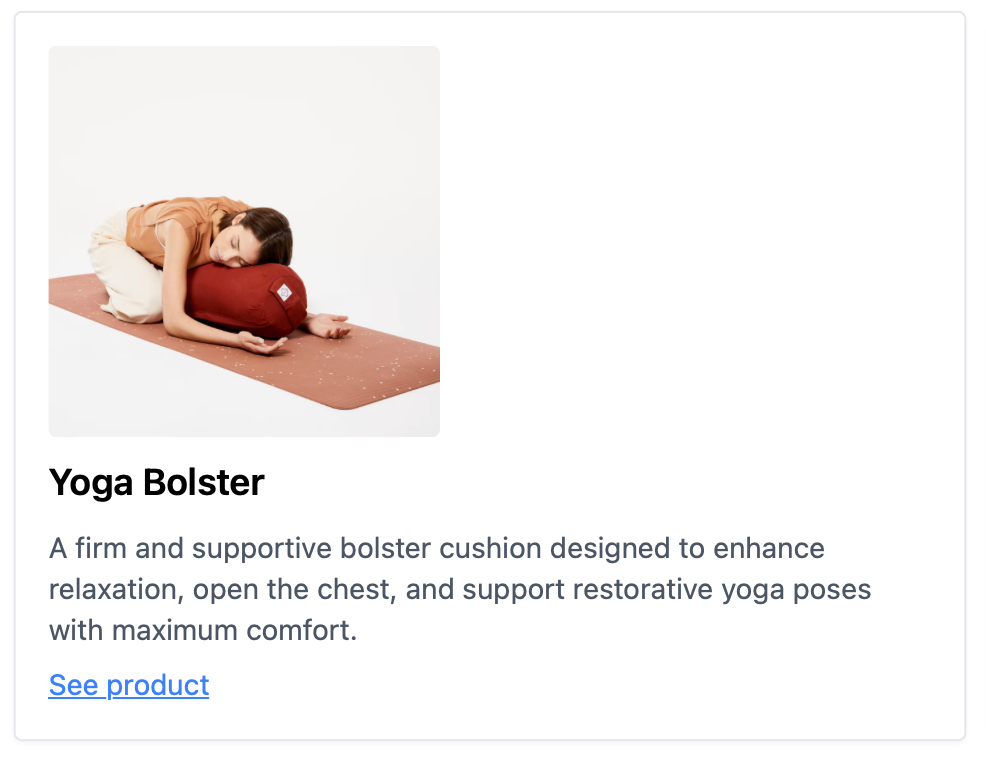
\includegraphics[width=0.2\textwidth]{asset/equipmentCard}
    \caption{\texttt{EquipmentCard}}
\end{figure}
\input{tech_content/documentation/custom_components/cards/teacher_card}
\paragraph{\texttt{FeedbackCard}}  \mbox{}\\

This component presents a card for a specific feedback, encompassing the name of the student who authored it, the comment, and the date of publication.
Prior to \texttt{CourseCard}, the first table of is relatively straightforward.


\begin{center}
    \begin{tabularx}{\textwidth}{|X|X|X|X|}
        \hline
        \textbf{Prop} & Type & Required & Description \\
        \hline
        \texttt{feedback} & \texttt{Feedback} & yes & A yoga feedback \\
        \hline
    \end{tabularx}
\end{center}

And more precisely

%\begin{center}
%    \begin{tabularx}{\textwidth}{|X|X|X|}
%        \hline
%        \textbf{Prop.attribute} & Type & Description \\
%        \hline
%        \texttt{feedback.photo} & \texttt{string | null} &  the path of  the yoga feedback's profile photo stored in Supabase\\
%        \hline
%        \texttt{feedback.name} & \texttt{string} & the name of the yoga feedback\\
%        \hline
%        \texttt{feedback.biography} & \texttt{string} & the biography of the feedback\\
%        \hline
%        \texttt{feedback.certificates} & \texttt{string[]} & a list of yoga certifications\\
%        \hline
%    \end{tabularx}
%\end{center}

\begin{figure}[H]
    \centering
    
\includegraphics[width=0.4\textwidth]{asset/feedbackCard}
    \caption{\texttt{feedbackCard}}
\end{figure}


\subsubsection{Navigation}

\paragraph{\texttt{Navbar}}  \mbox{}\\


This component serves as the navigation bar of the web application, encompassing all its key landmarks. Its layout
undergoes a significant transformation in accordance with the maximum available screen width.




\begin{figure}[H]
    \centering
    
\includegraphics[width=0.9\textwidth]{asset/navbar}
    \caption{\texttt{Navbar}}
\end{figure}

\begin{figure}[H]
    \centering
    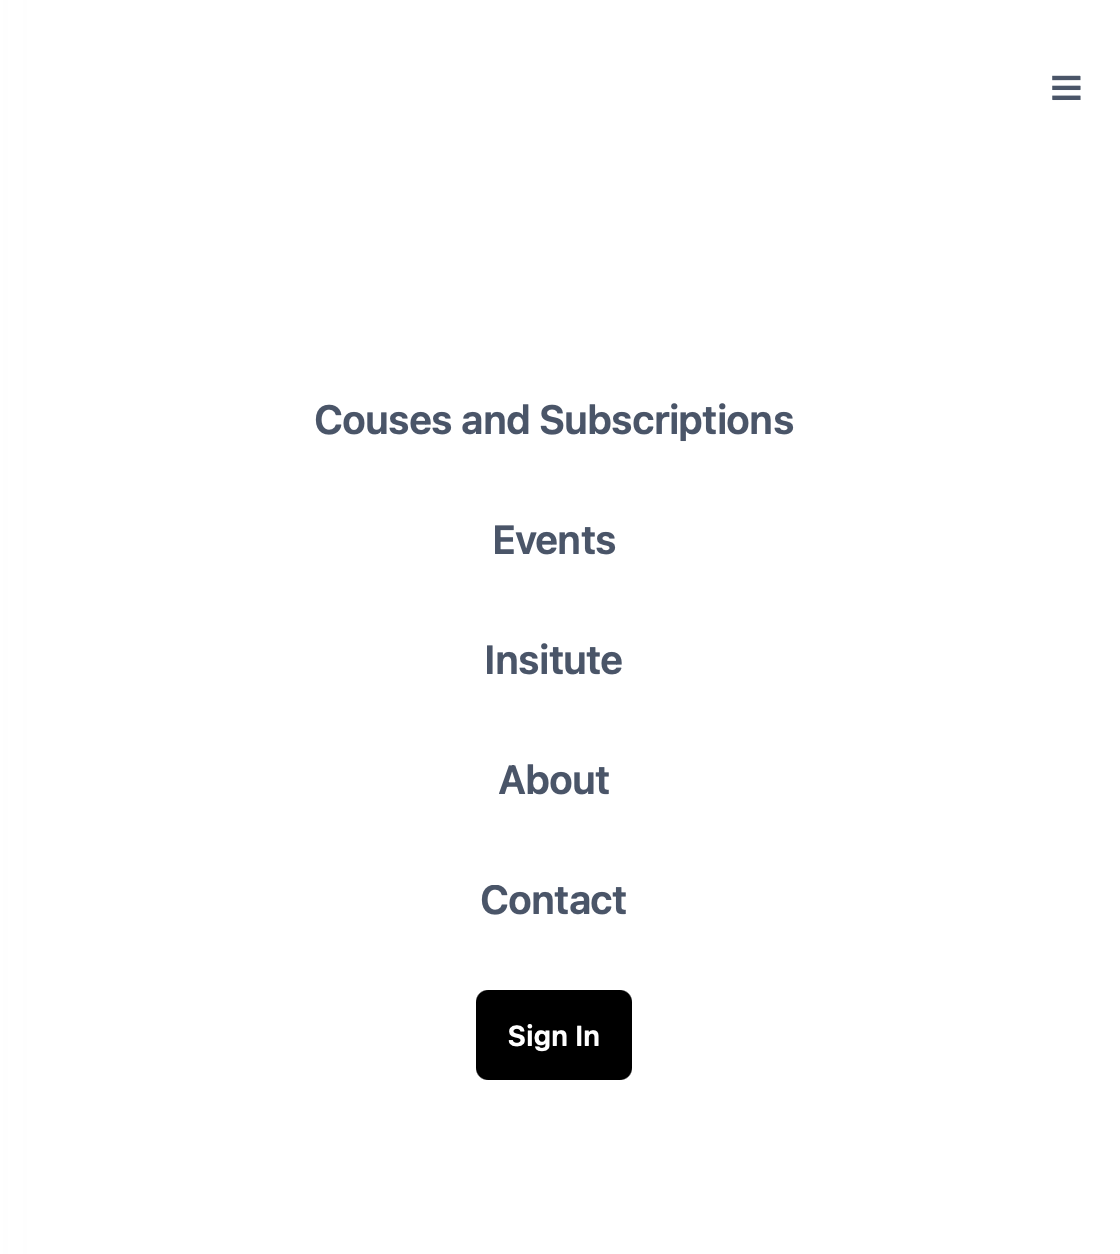
\includegraphics[width=0.4\textwidth]{asset/navbarResponsive_2}
    \caption{\texttt{Navbar for mobile devices}}
\end{figure}
\paragraph{\texttt{Footer}}  \mbox{}\\


This component serves as the footer of the web application, providing a comprehensive list of landmarks and essential links.





\subsubsection{User interaction}
\paragraph{\texttt{BaseLinkButton}} \mbox{}\\

This component renders either a clickable button or a NuxtLink, depending on the props passed to it. It supports
multiple visual variants and handles both real navigation and fake/dummy behavior. The component is useful for
consistent call-to-action buttons and links across the application.

\begin{center}
    \begin{tabularx}{\textwidth}{|X|X|X|X|}
        \hline
        \textbf{Prop} & Type & Required & Description \\
        \hline
        \texttt{url} & \texttt{string} & no & The link target if used as a NuxtLink \\
        \hline
        \texttt{variant} & \texttt{number} & no & Defines the visual style (1 to 4 variants available) \\
        \hline
        \texttt{asButton} & \texttt{boolean} & no & Forces rendering as a \texttt{<button>} even if \texttt{url} is set and not \texttt{NuxtLink} \\
        \hline
        \texttt{disabled} & \texttt{boolean} & no & Disables the button (only effective when \texttt{asButton} is \texttt{true}) \\
        \hline
    \end{tabularx}
\end{center}

\paragraph{Emits}
\begin{itemize}
    \item \texttt{click} – Emitted when the button is clicked (only if rendered as a \texttt{<button>})
\end{itemize}

Moreover, both versions (the \texttt{<button>} and the \texttt{NuxtLink}) include a default slot to embed custom HTML content.



\begin{figure}[H]
    \centering
    \begin{minipage}[b]{0.32\textwidth}
        \centering
        
\includegraphics[width=\textwidth]{asset/firstButton}
    \end{minipage}
    \hfill
    \begin{minipage}[b]{0.32\textwidth}
        \centering
        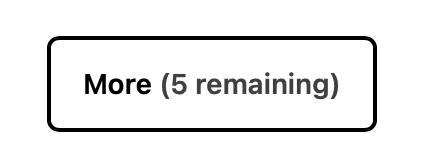
\includegraphics[width=\textwidth]{asset/secondButton}
    \end{minipage}
    \hfill
    \begin{minipage}[b]{0.32\textwidth}
        \centering
        
\includegraphics[width=\textwidth]{asset/thirdButton}
    \end{minipage}
    \caption{\texttt{All the buttons (Primary - Secondary - Third)}}
\end{figure}


\paragraph{\texttt{FormInput}}  \mbox{}\\


This component renders a labeled input field with validation feedback. It is designed for use in forms and supports binding with \texttt{v-model} via the \texttt{modelValue} prop. The label and input are semantically linked using the \texttt{id} attribute. Error messages can be displayed below the input when validation fails.

\begin{center}
    \begin{tabularx}{\textwidth}{|X|X|X|X|}
        \hline
        \textbf{Prop} & Type & Required & Description \\
        \hline
        \texttt{id} & \texttt{string} & yes & Unique identifier for the input, used to associate the label \\
        \hline
        \texttt{modelValue} & \texttt{string} & no & The current value of the input (used with \texttt{v-model}) \\
        \hline
        \texttt{label} & \texttt{string} & yes & The text displayed in the label above the input \\
        \hline
        \texttt{type} & \texttt{string} & no & The HTML input type (e.g., \texttt{text}, \texttt{email}, \texttt{password}) \\
        \hline
        \texttt{placeholder} & \texttt{string} & no & Placeholder text inside the input field \\
        \hline
        \texttt{required} & \texttt{boolean} & no & Whether the input is required \\
        \hline
        \texttt{error} & \texttt{string} & no & Displays a red error message below the input if set \\
        \hline
    \end{tabularx}
\end{center}

\paragraph{Emits}
\begin{itemize}
    \item \texttt{update:modelValue} – Emitted on every input change to update the bound model
\end{itemize}



\begin{figure}[H]
    \centering
    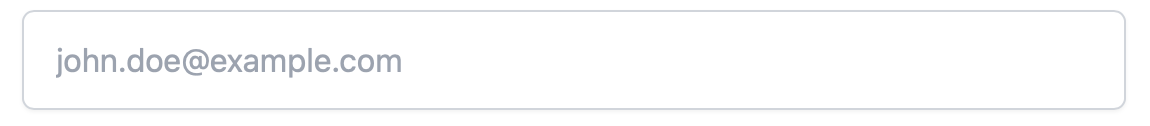
\includegraphics[width=0.7\textwidth]{asset/formInput}
    \caption{\texttt{FormInput}}
\end{figure}

\paragraph{\texttt{BreadcrumbTrail}} \mbox{}\\

This component displays a horizontal breadcrumb navigation trail composed of up to three levels. It uses \texttt{NuxtLink} elements for navigation when possible and shows a plain text label for the final level if present. Each breadcrumb is visually separated by a \texttt{>} character.

\begin{center}
    \begin{tabularx}{\textwidth}{|X|X|X|X|}
        \hline
        \textbf{Prop} & Type & Required & Description \\
        \hline
        \texttt{breadCrumbs} & \texttt{Array<{ name: string, link: string }>} & no & An array of breadcrumb items (up to 3). The first two items are shown as links; the third, if present, is rendered as plain text. \\
        \hline
    \end{tabularx}
\end{center}

\paragraph{Structure and Behavior}
\begin{itemize}
    \item The first two elements in \texttt{breadCrumbs} are rendered as clickable \texttt{NuxtLink}s.
    \item If a third element exists, it is rendered as plain text to indicate the current page.
    \item Separators (\texttt{>}) are inserted between breadcrumb levels using styled \texttt{<p>} elements.
\end{itemize}


\begin{figure}[H]
    \centering
    
\includegraphics[width=0.7\textwidth]{asset/breadcrumb}
    \caption{\texttt{Breadcrumb} with two navigable links and a third current page label}
\end{figure}




